\section{EBS}\label{sec:ebs}

\subsection{What is}\label{subsec:what-is-ebs}
EBS (Elastic Block Store) Volume is a network drive that can be attached to a EC2 while they run. EBS can only be \textbf{assigned to one EC2 at a time}, they it is bound to a \textbf{specific availability zone} and it has a provisioned capacity in GBs and IOPS.

\subsection{EBS Snapshots}\label{subsec:ebs-snapshots}
Snapshots are \textbf{backups a EBS Volume at a point in time}, and can be copied across regions/AZ. Since you cannot move an EBS across regions/AZ, you can create a Snapshot in the region, and then create a new EBS from the snapshot in the desired region/AZ.

\begin{figure}[h]
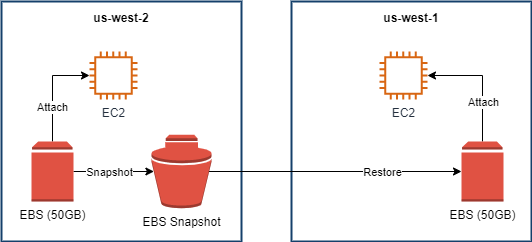
\includegraphics[scale=0.5]{ebs/ebs}
\centering\label{fig:ebs}
\end{figure}

\subsection{AMI}\label{subsec:ami}
It stands for Amazon Machine Image and are a \textbf{customization} of an EC2 instance (With additional software, config, OS, etc). they are built for a \textbf{specific region} but can be copied across regions.
You can launch EC2 instances from:
	\begin{itemize}
		\item{Public AMI (AWS provided)}
		\item{Your own AMI (maintained by you development team}
		\item{AWS Marketplace AMI (Someone else's AMI)}
	\end{itemize}

\subsection{EC2 Instance Store}\label{subsec:ec2-instance-store}
\textbf{Ephemeral storage} (Data is lost upon restart) that is located in the same physical location of the EC2 instance and provides a \textbf{better I/O performance}. It's good for buffering and caching but it's \textbf{more expensive}.

\subsection{EFS}\label{subsec:efs}
Managed NFS (network file system) that \textbf{can be bond to multiple EC2 across multiple AZ}. It is \textbf{HA, scalable and very expensive}.

\subsection{EC2 Storage Shared responsibility model}\label{subsec:ec2-storage-shared-responsibility-model}
\begin{itemize}
	\item{Setting backup / snapshot procedures}
	\item{Setting up data encryption}
	\item{Responsibility of any data on the volumes}
	\item{Understand the risk of using EC2 Instance Store}
\end{itemize}